\subsection{两条直线的位置关系}\label{subsec:1-4}

我们知道,在同一个平面内的两条直线\footnotemark 的位置关系只有两种:平行或相交。
\footnotetext{本书中没有特别说明的“两条直线(平面)”,均指不重合的两条直线(平面)。}

空间的两条直线之间,还有另外一种位置关系。

观察图 \ref{fig:ltjh-1-11} 中的六角螺母的棱 $AB$ 和 $CD$ 所在的直线,或机械部件蜗轮和蜗杆的轴线,
可以看出,它们不同在一个平面内。

\begin{figure}[htbp]
    \centering
    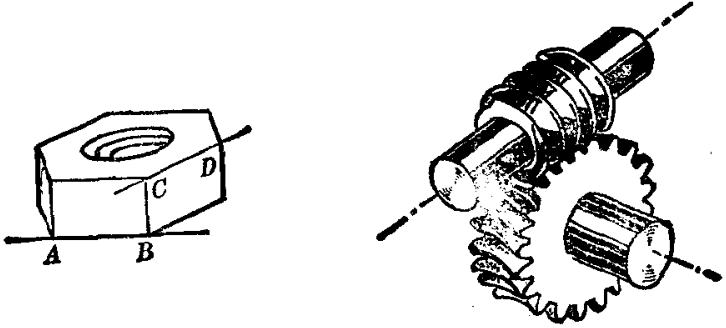
\includegraphics[width=10cm]{../pic/ltjh-ch1-11.png}
    \caption{}\label{fig:ltjh-1-11}
\end{figure}

我们把不同在任何一个平面内的两条直线叫做\zhongdian{异面直线}。
显然,两条异面直线是既不平行又不相交的。

空间的两条直线的位置关系有以下三种:

(1)\zhongdian{相交直线} —— 在同一个平面内,有且只有一个公共点;

(2)\zhongdian{平行直线} —— 在同一个平面内,没有公共点;

(3)\zhongdian{异面直线} —— 不同在任何一个平面内,没有公共点。

画异面直线时,可以画成如图 \ref{fig:ltjh-1-12} 那样,以显示出它们不共面的特点。

\begin{figure}[htbp]
    \centering
    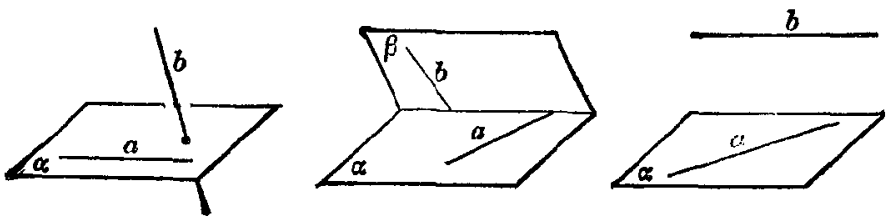
\includegraphics[width=11cm]{../pic/ltjh-ch1-12.png}
    \caption{}\label{fig:ltjh-1-12}
\end{figure}

直线 $a$、$b$ 相交于点 $A$,我们规定记作 $a \cap b = A$。

\liti[0] \zhongdian{平面内一点与平面外一点的连线,和平面内不经过该点的直线是异面直线。}

\begin{wrapfigure}[8]{r}{5cm}
    \centering
    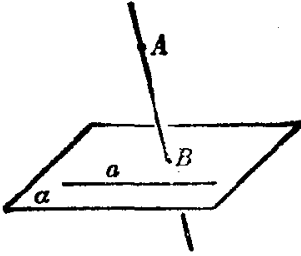
\includegraphics[width=4cm]{../pic/ltjh-ch1-13.png}
    \caption{}\label{fig:ltjh-1-13}
\end{wrapfigure}

已知:$a \subset \alpha$, $A \not \in \alpha$, $B \in \alpha$, $B \not \in a$。(图 \ref{fig:ltjh-1-13})。

求证:直线 $AB$ 和 $a$ 是异面直线。

\zhengming 假设直线 $AB$ 与 $a$ 在同一个平面内,那么这个平面一定经过点 $B$ 和直线 $a$。

$\because$ \quad $B \not \in a$, 经过点 $B$ 与直线 $a$ 只能有一个平面 $\alpha$,

$\therefore$ \quad 直线 $AB$ 与 $a$ 应在平面 $\alpha$ 内。

$\therefore$ \quad $A \in \alpha$, 这与已知 $A \not \in \alpha$ 矛盾。

$\therefore$ \quad 直线 $AB$ 和 $a$ 是异面直线。


\begin{lianxi}

\xiaoti{在教室里找出几对异面直线的例子。}

\xiaoti{}%
\begin{xiaoxiaotis}%
    \xxt[\xxtsep]{没有公共点的两条直线叫做平行直线。对吗?}

    \xxt{分别在两个平面内的两条直线一定是异面直线吗?为什么?}

\end{xiaoxiaotis}

% TODO: wrapfigure 在这里无法正常使用
\begin{minipage}{7cm}
    \jiange
    \xiaoti{说出正方体中各对线段的位置关系:}
    \begin{xiaoxiaotis}

        \xxt{$AB$ 和 $CC_1$;}

        \xxt{$A_1C$ 和 $BD_1$;}

        \xxt{$A_1A$ 和 $CB_1$;}

        \xxt{$A_1C_1$ 和 $CB_1$;}

        \xxt{$A_1B_1$ 和 $DC$;}

        \xxt{$BD_1$ 和 $DC$。}

    \end{xiaoxiaotis}
\end{minipage}
\quad
\begin{minipage}{4cm}
    \centering
    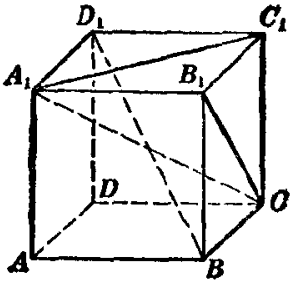
\includegraphics[width=3.5cm]{../pic/ltjh-ch1-subsec4-lx-03.png}\\
    (第 3 题)
\end{minipage}

\end{lianxi}

